\subsubsection{Variable Geometry Screws Origami}
\label{sec:screwdrive_variable_pitch}

\begin{figure}[htb]
    \begin{subfigure}{0.5\textwidth}
    \centering
    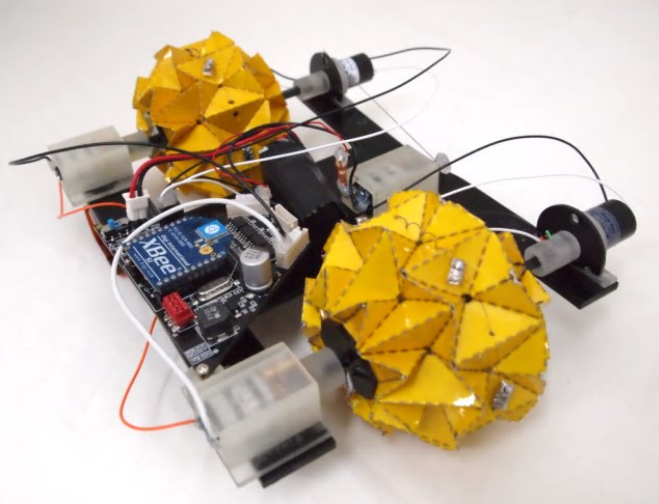
\includegraphics[width=.90\columnwidth]{images/origami_lee2013.png}
    \caption{Deformable wheel robot, \cite{Lee2013}.}
    %\vspace{-20pt}
    \label{fig:origami_lee}
    \end{subfigure}
    \begin{subfigure}{0.5\textwidth}
    \centering
    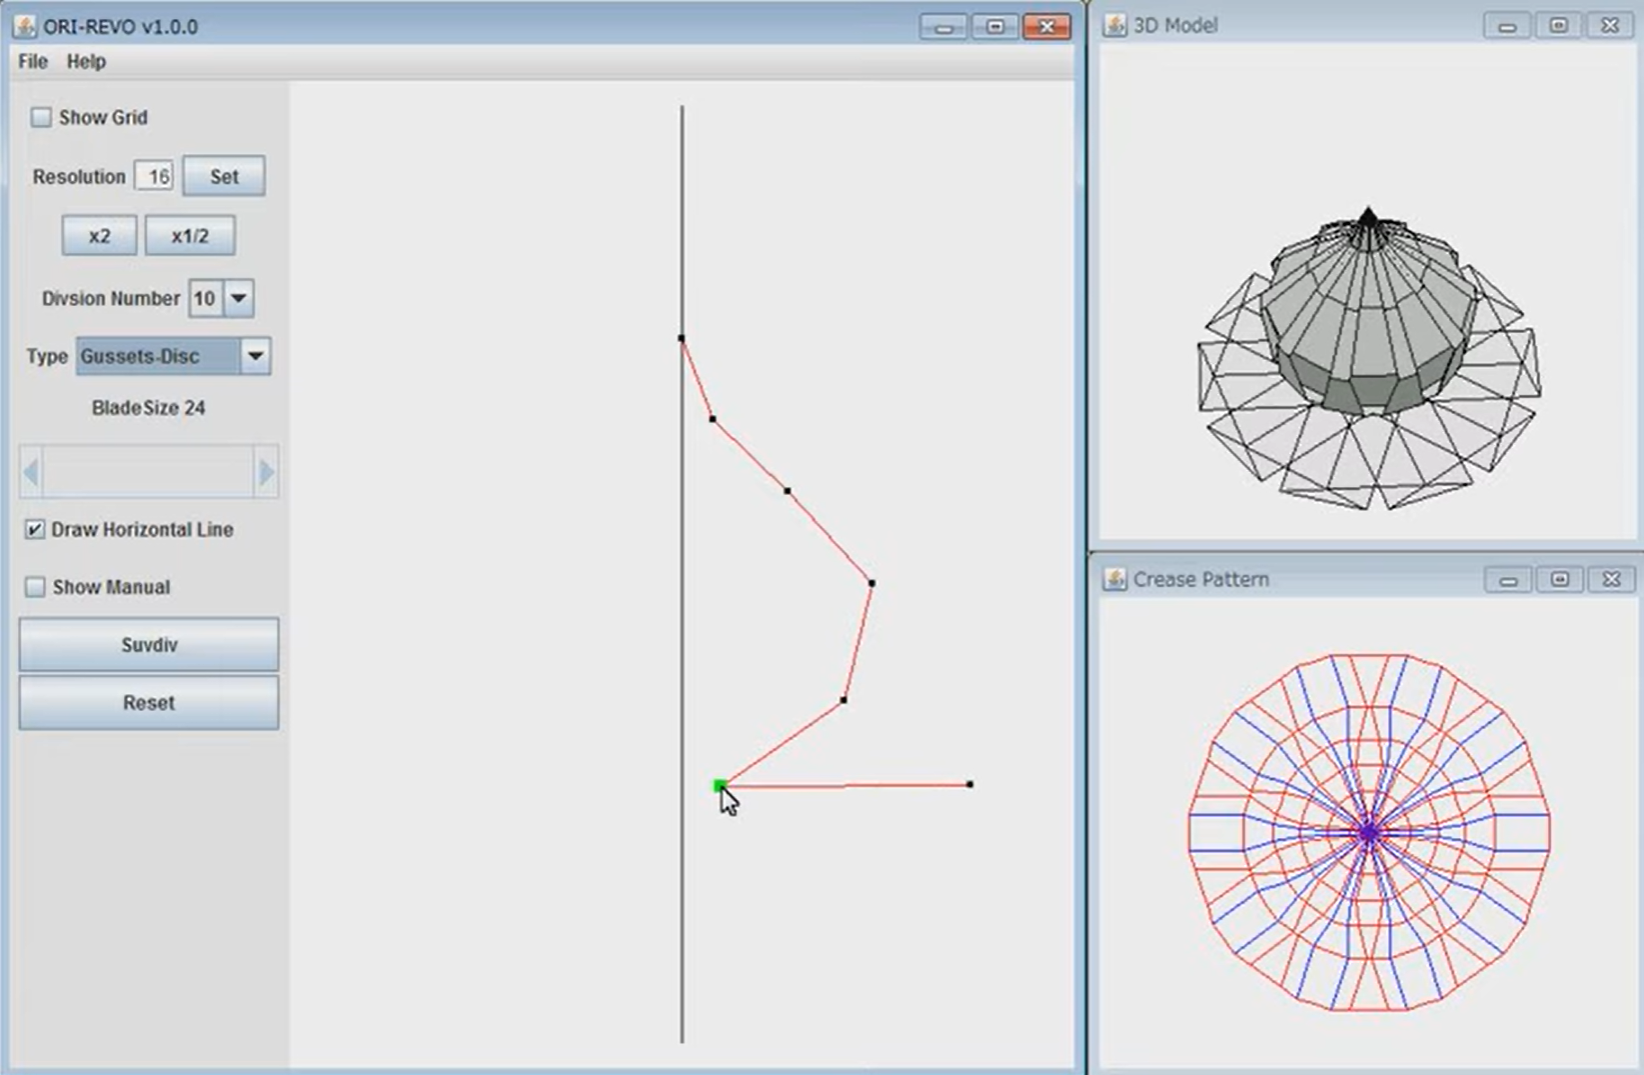
\includegraphics[width=1.10\columnwidth]{images/origami_orirevo.png}
    \caption{ORI-REVO software, \cite{Mitani2009}.}
    %\vspace{-20pt}
    \label{fig:origami_orirevo}
    \end{subfigure}
    \caption{Origami applications and software}
    \label{fig:origami_lee_orirevo}
\end{figure}

%\begin{figure}[!htb]
    %\centering
    %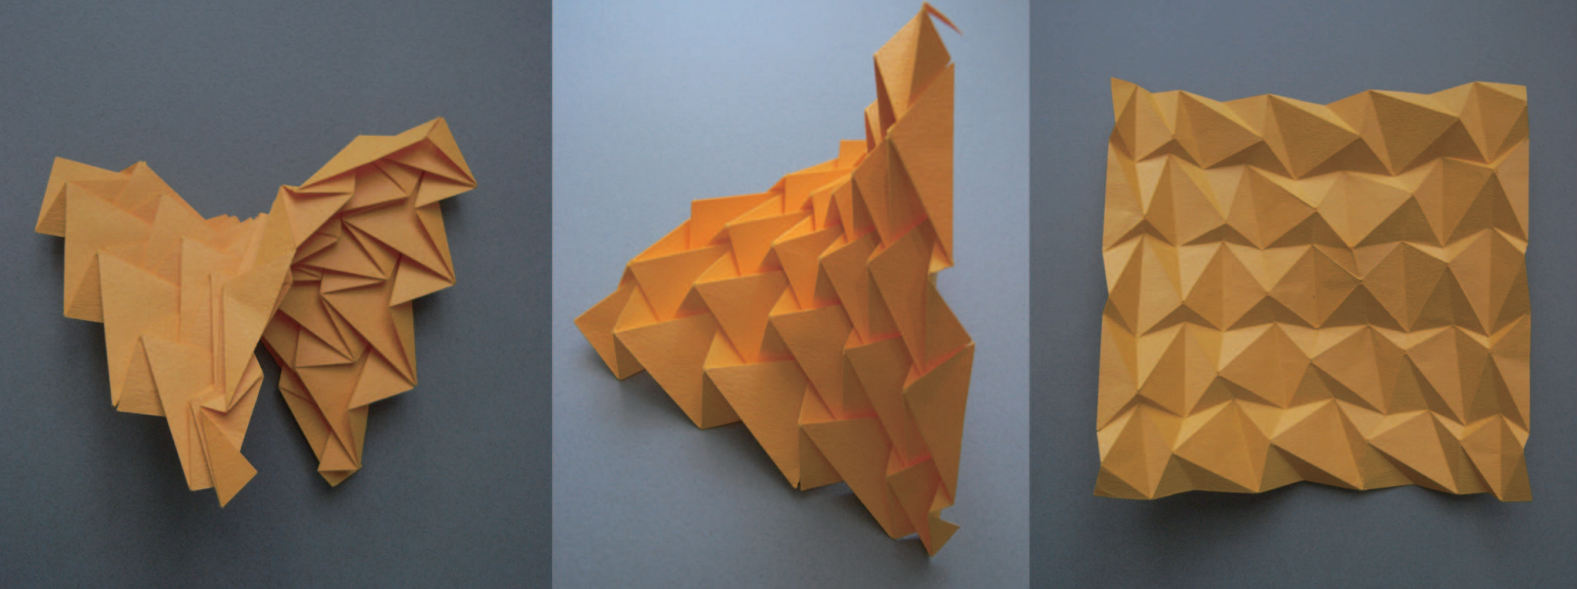
\includegraphics[width=.90\columnwidth]{images/origami_tachi2010_complex_real.png}
    %\caption{Origami structures, \cite{Tachi2010}.}
    %\vspace{-20pt}
    %\label{fig:origami_tachi_complex_real}
%\end{figure}


%Motivation
Once optimal screw parameters for a given set of terrains are found and an onboard terrain classification system provides the type of terrain, a variable pitch screw would allow switching between different sets of geometries to best suit the terrain. 

Origami is an art form that is increasingly being looked to for its ability to create folding structures from a two dimensional pattern, from MEMS devices \cite{yan2016}, to robotic crawling actuators \cite{Rafsanjani2018}, to deformable wheels \cite{Lee2013}, and medical microrobots \cite{Miyashita2015} this technique allows creation of metamaterials that can be actuated with a single degree of freedom. In metamaterials, the resulting structure depends not only on the underlying construction material, but also the geometry, leading to structures that can exhibit wildly different properties, such as stiffness, compressive moduli, etc, than their base material. 

Current fabrication methods for the screws utilize three dimensional printing. While useful for initial prototypes, utilizing a laser cutter would decrease fabrication time significantly as Silverberg et al. \cite{Silverberg2015} and Rafsanjani \cite{Rafsanjani2018} have found. Furthermore, this fabrication method could provide the means by which to design and fabricate a robust variable pitch screw with a high degree of robustness as compared to an articulated variable pitch device. 

%Furthermore, generating origami via traditional hand-folding methods, while simple, creates pre-creases in the material that are not necessary in the final structure but are nevertheless present and affect stiffness, adding additional degrees of freedom to the structure. 

%In \cite{Silverberg2014a} Silverberg utilized dash-and-gap perforations since it was found that continuous line patterns lead to lattices that are easy to tear and exhibit anisotropic bending properties. Dash-and-gap, on the other hand, allowed isotropic bending properties and equal folding stiffness for valley and mountain creases. Another form of manufacture would be a two step process where the laser would make engravings of mountain or valley folds instead of cutting all the way through. This would lead to a stronger and sealed surface which is desirable ingress protection. 

Lee et al.\cite{Lee2013} create an active origami wheel using the waterbomb, or magic ball, origami pattern for the structure and a combination of passive elements, such as a spring, and smart wire actuators to achieve changes in its shape, Figure ~\ref{fig:origami_lee}. Silverberg et al. \cite{Silverberg2015} utilize the Miura-ori tesselated folding pattern to create structures comprised of individual cells that are bistable, that is they settle into decreased energy minima. This switchable behavior would be pertinent in actuator design as it would allow structures that have two stable passive states with energy needed only to switch states. 

%The magic ball pattern is comprised of individual unit structures, in this case triangles, that exhibit independent behavior but can be chained to produce a bulk structure composed of individual switchable units, as in Figure ~\ref{fig:origami_lee}. 


%Furthermore, they showed that many structures can arise from the same underlying patterns by localized push-through-defects. One could imagine a robot hull made of a Miura-ori tesselated surface where each unit cell is actuated via an individual actuator to change the outer structure of the robot in real-time. 

%\begin{figure}[!htb]
    %\centering
    %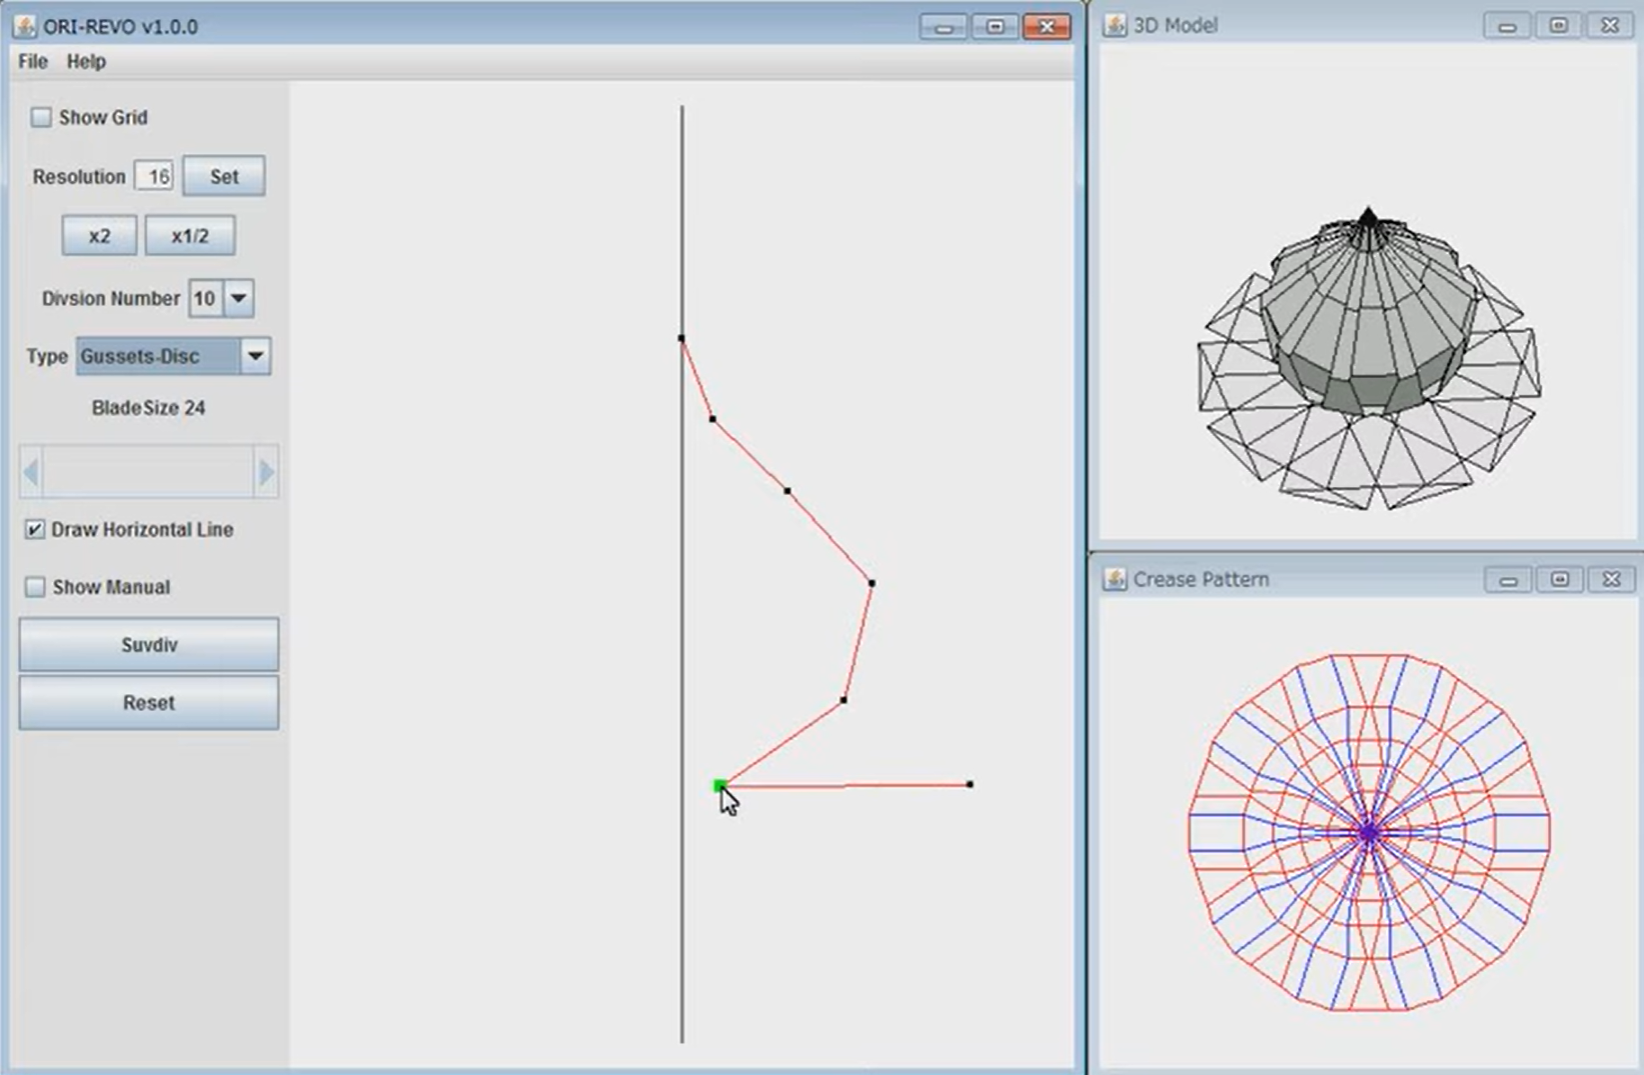
\includegraphics[width=.90\columnwidth]{images/origami_orirevo.png}
    %\caption{ORI-REVO software, \cite{Mitani2009}.}
    %\vspace{-20pt}
    %\label{fig:origami_orirevo}
%\end{figure}



With this project, we propose development of a screw using origami principles to achieve an actuatable surface capable of transitioning between two distinct stable configurations and where the limits are set either mechanically or by exploiting origami bistability. 

% inverse design problem 
In order to do this a crease pattern needs to be generated to create the target design, this is known as the inverse design problem. Castle et al. \cite{Castle2014} programatically tackle the inverse problem of designing cuts and folds in a 2D surface to obtain a given 3D object. The justification of the cuts is that there are features that can be obtained more effectively by removing material.  


Boyle et al. created a complex double curvature three dimensionaly face from an initially flat 3D-printed surface. This is known as shape-morphing or active origami principles, there the morphing occurs due to an external stimuli, such as pneumatics or, in this case, temperature differences. 3D inverse design was used to specify the target shape and then work backwards to program the metamaterial. 	

Mitani et al. \cite{Mitani2009} created the ORI-REVO software which allows creation of revolution surfaces by specifying a profile pattern, see Figure ~\ref{fig:origami_orirevo}. This tool also allows the specification of division number, resolution, as well as manual manipulation in real time. The resultant 3D form is shown in the top right and the crease pattern in the bottom right. %rotational symmetry


Morever actuation forces need to be computed in order to specify the actuator. Fuchi et al. \cite{Fuchi2013} have developed OMTO (an origami modeling toolbox for matlab) which uses FEM to set boundary conditions, fixed points, and forced point to calculate fold lines that optimize greatest displacement in specified directions at the output nodes. In 2018, Gillman \cite{Gillman2018} continued this work adding nonlinear optimization yet removing the graphical user interface. 





%\begin{figure}[htb]
    %\centering
    %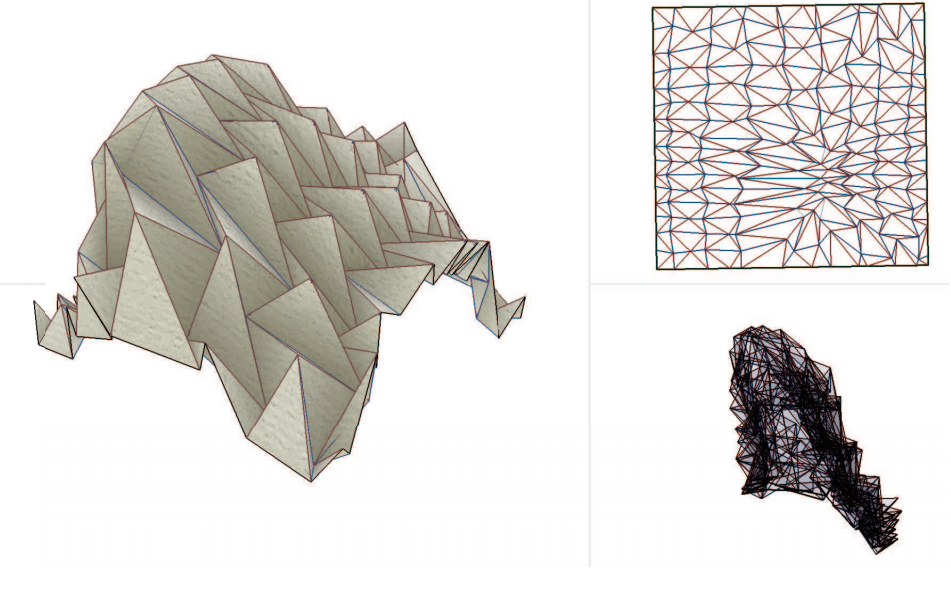
\includegraphics[width=.90\columnwidth]{images/origami_tachi2010_complex_pattern.png}
    %\caption{Complex origami forms, \cite{Tachi2010}.}
    %\vspace{-20pt}
    %\label{fig:origami_tachi_complex_pattern}
%\end{figure}









%%% MERGE ABOVE AND BELOW


%\begin{figure}[htb]
    %\centering
    %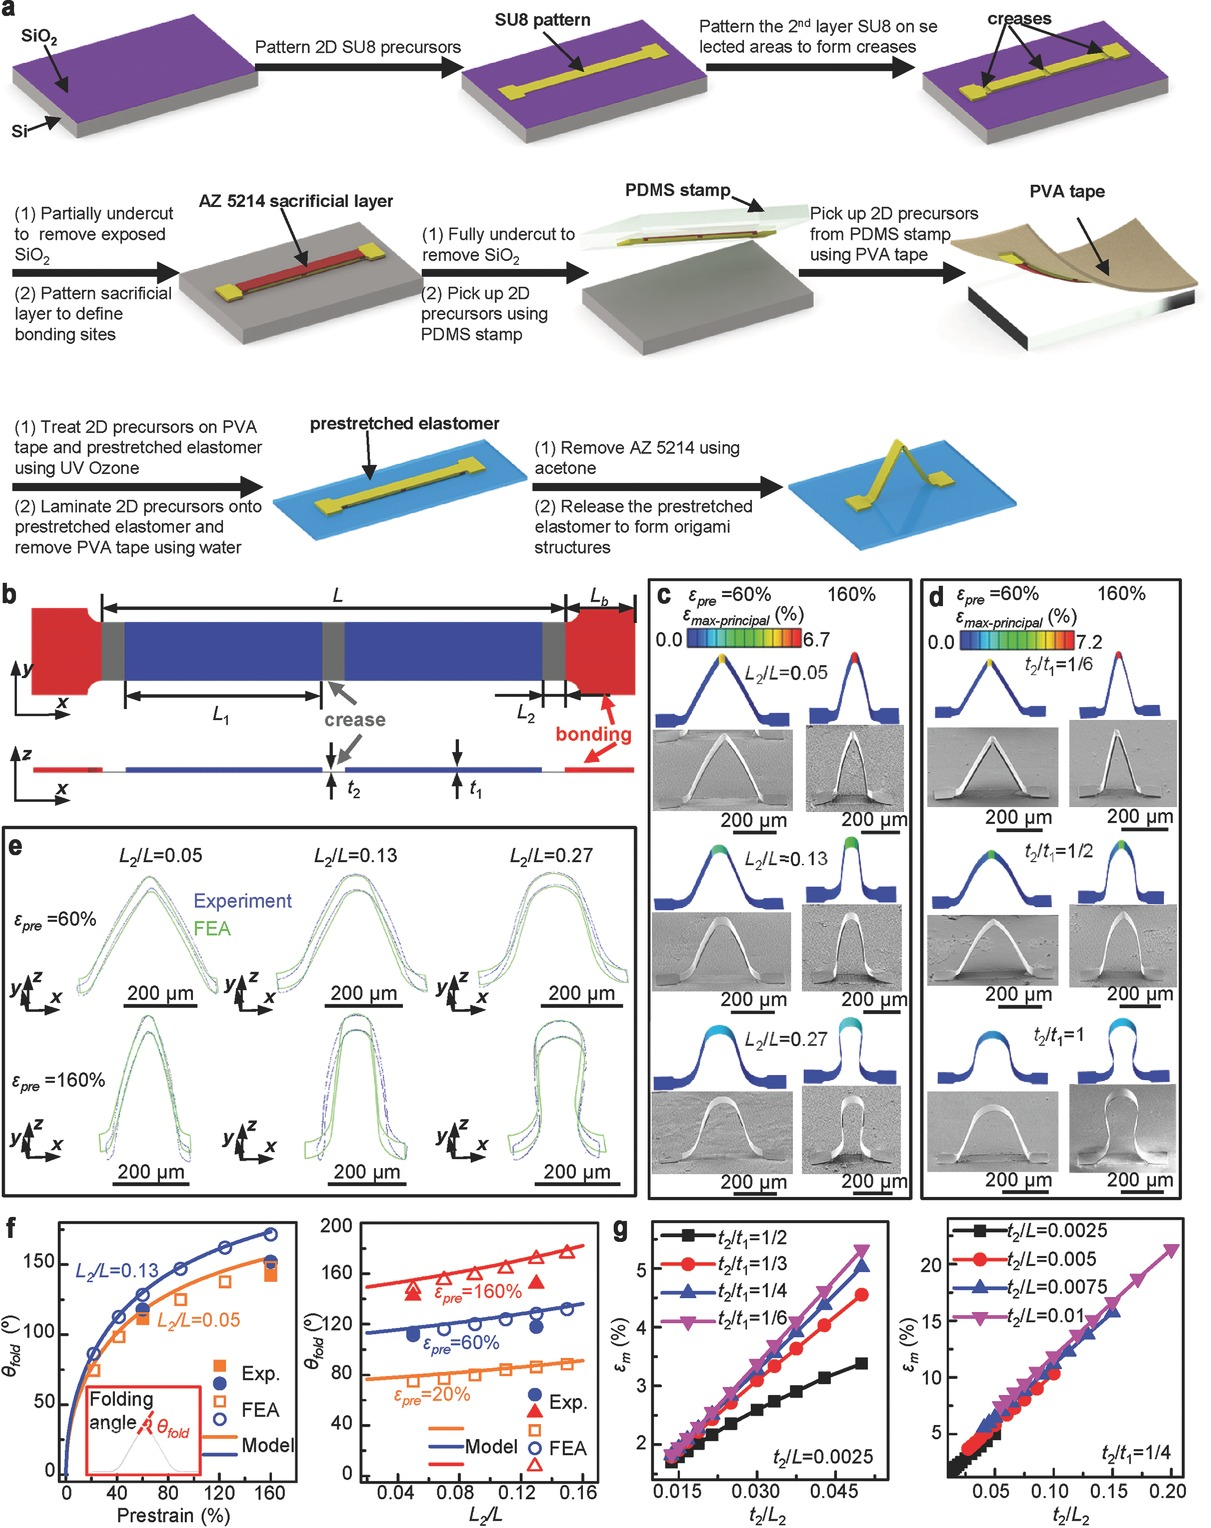
\includegraphics[width=.90\columnwidth]{images/lit_review/yan2016_origami_mems_folds.jpg}
    %\caption{Controlled Mechanical Buckling for Origami‐Inspired Construction of 3D Microstructures in Advanced Materials, \cite{yan2016}.}
    %\vspace{-20pt}
    %\label{fig:origami_mems}
%\end{figure}

%\begin{figure}[htb]
    %\centering
    %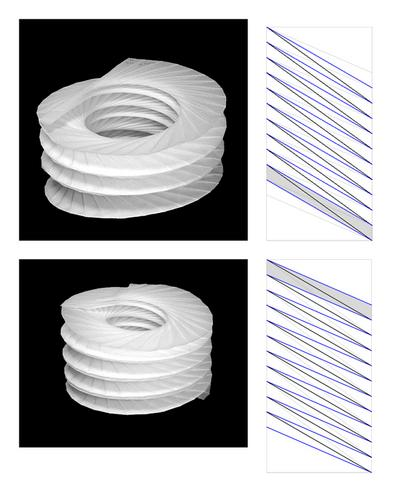
\includegraphics[width=.90\columnwidth]{images/lit_review/azuma_origami_convolution.jpg}
    %\caption{Azumi et al.'s convolutional helix, \cite{yan2016}.}
    %\vspace{-20pt}
    %\label{fig:origami_mems}
%\end{figure}


%computational origami https://langorigami.com/article/computational-origami/ 

%\emph{Programmability of the lattice expansion}
%Programmability of the lattice expansion to redirect force exerted by screws on land due to a morphed geometry. This programmability has been demonstrated by Rafsanjani et al \cite{Rafsanjani2018} in which they programmed their actuator's expansion as is required to achieve a snake like crawl, in which some scales contract while others expand, leading to overall positive net displacement. 
%
%Photo of snake actuator. 
%Bistability
%Methods
%Laser cut of valley and mountain folds
%Image of laser cut delrin
%Itae Cohen's supplemental material? 
%%Algorithms?laser


%Software: ORI-REVO
%" This software is a design software that allows users to interact with origami forms while altering the crease pattern of the model. The software can keep: Developability (foldable from a piece of paper) Flat-foldability (foldable into a flat shape) Planarity of facets (paper do not twist in 3D form) Point coordinate coincidence Paper size "

% WATERBOMB FIGURE
%\begin{figure}[htb]
    %\centering
    %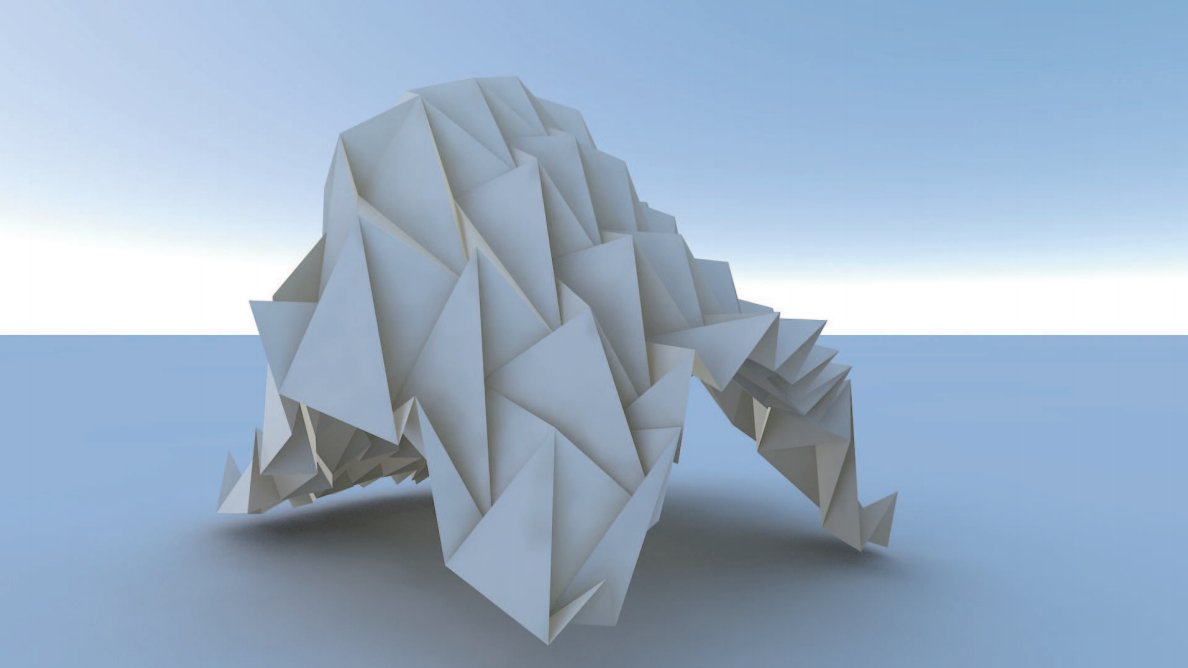
\includegraphics[width=.90\columnwidth]{images/origami_tachi2010_complex.png}
    %\caption{Waterbomb origami forms, \cite{Tachi2010}.}
    %\vspace{-20pt}
    %\label{fig:origami_tachi_complex}
%\end{figure}

